% Sample of a report for an attack as requested at wednesday, 5 December 2018, mail "Assignemnt Lab 19"
\subsection{IP Spoofing}
% Introduction about this attack
\subsection{Introduction}
In order to hide the IP address of a sender machine and at the same time identifying a station active on the network, an attacker could be use a method named \textit{IP spoofing}.\par
The IP spoofing consists to send ICMP packets with a fake source IP that isn't mapped on the network to recognize the reply of the active host connected to the network.\par

% SCAPY program
\subsubsection{SCAPY program}
In this scapy program the attacker has an IP that is not in the network (192.168.102.102) and it sends ICMP packets to all the host that could be present in the subnetwork 192.168.62.0/24.\par
\lstinputlisting{scapy/IPSpoofing.py}

% Wireshark presenting  the attacker's messages
\subsubsection{Attacker's messages}
%Wireshark filter: \textit{icmp \&\& ip.addr == 192.168.102.102}\par
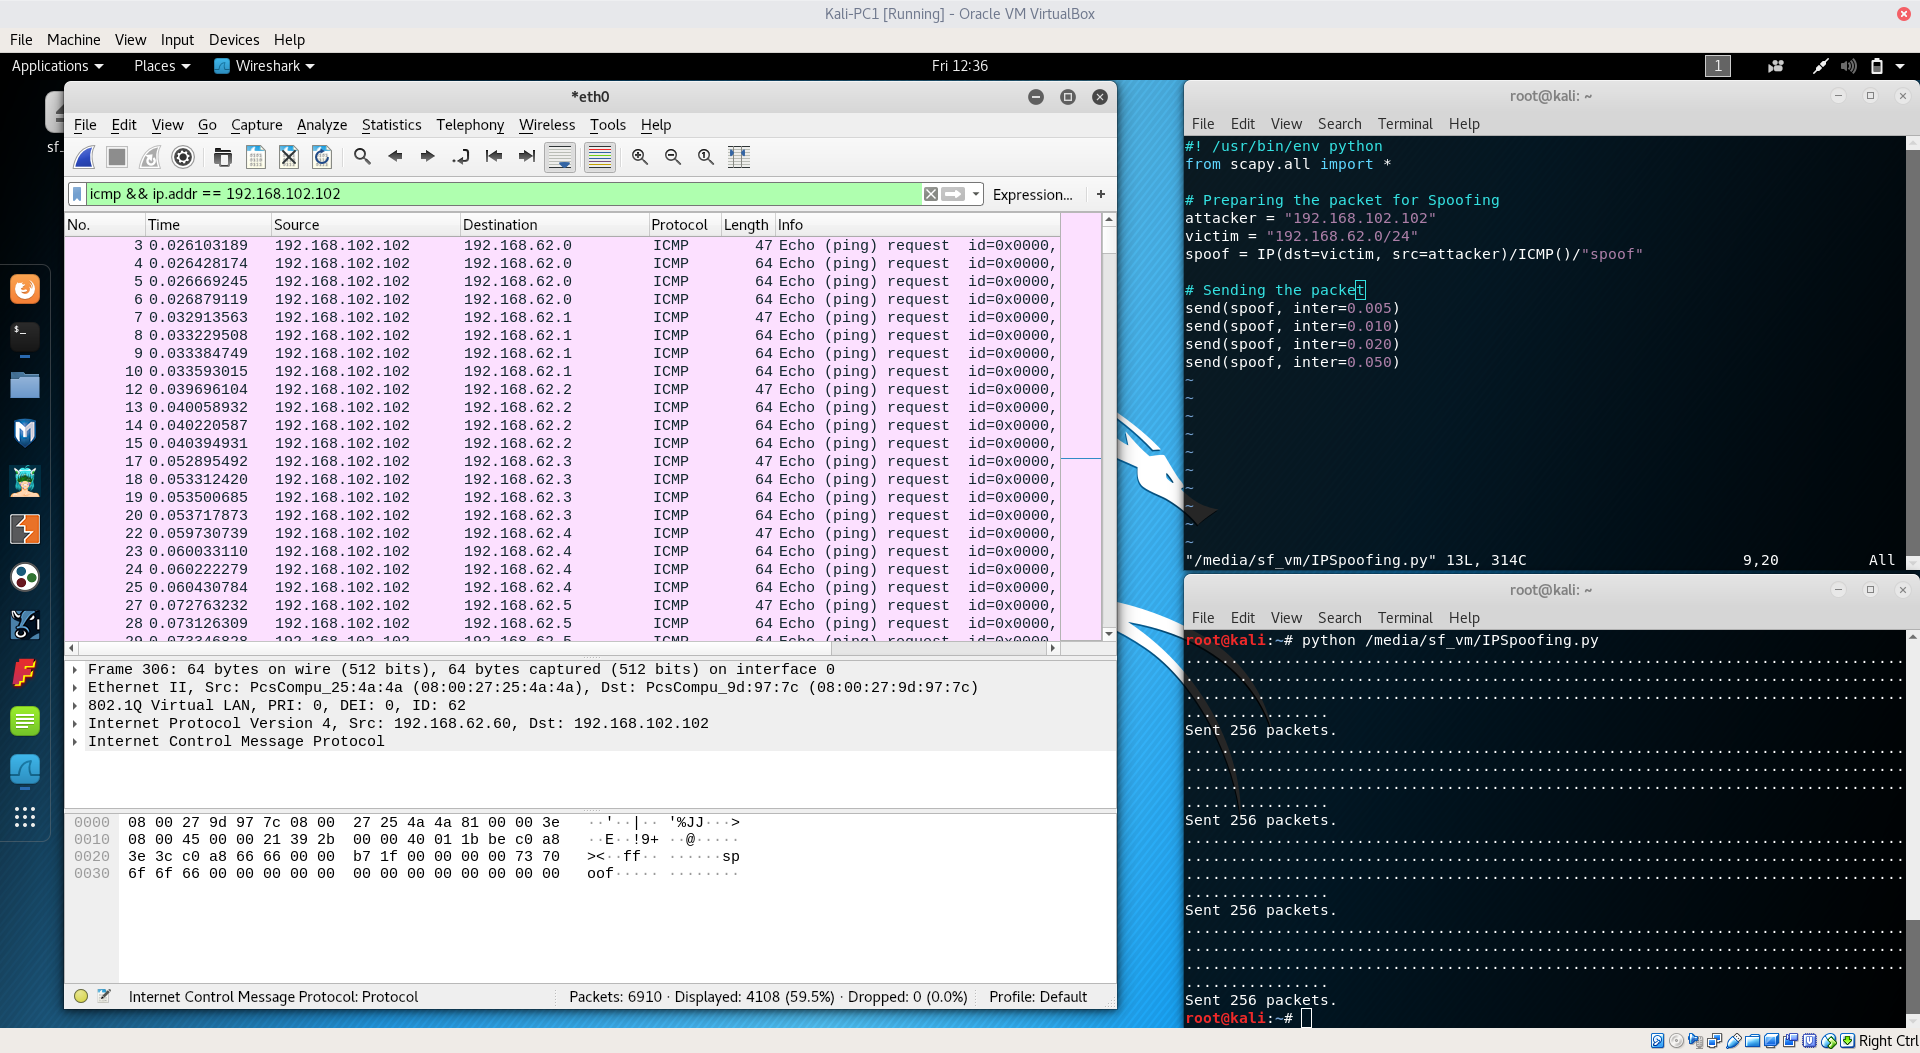
\includegraphics[width=16cm]{img/IPSpoofingICMP.png}

% Explanation of the result of the attack
\subsubsection{Attack's result}
Wireshark has received the ICMP reply packets of the host attacked. So the attacker had sent packets to the active host and the host hadn't recognized the real sender (the attacker).\par
%Wireshark filter: \textit{icmp.type == 0 \&\& ip.addr == 192.168.102.102}\par
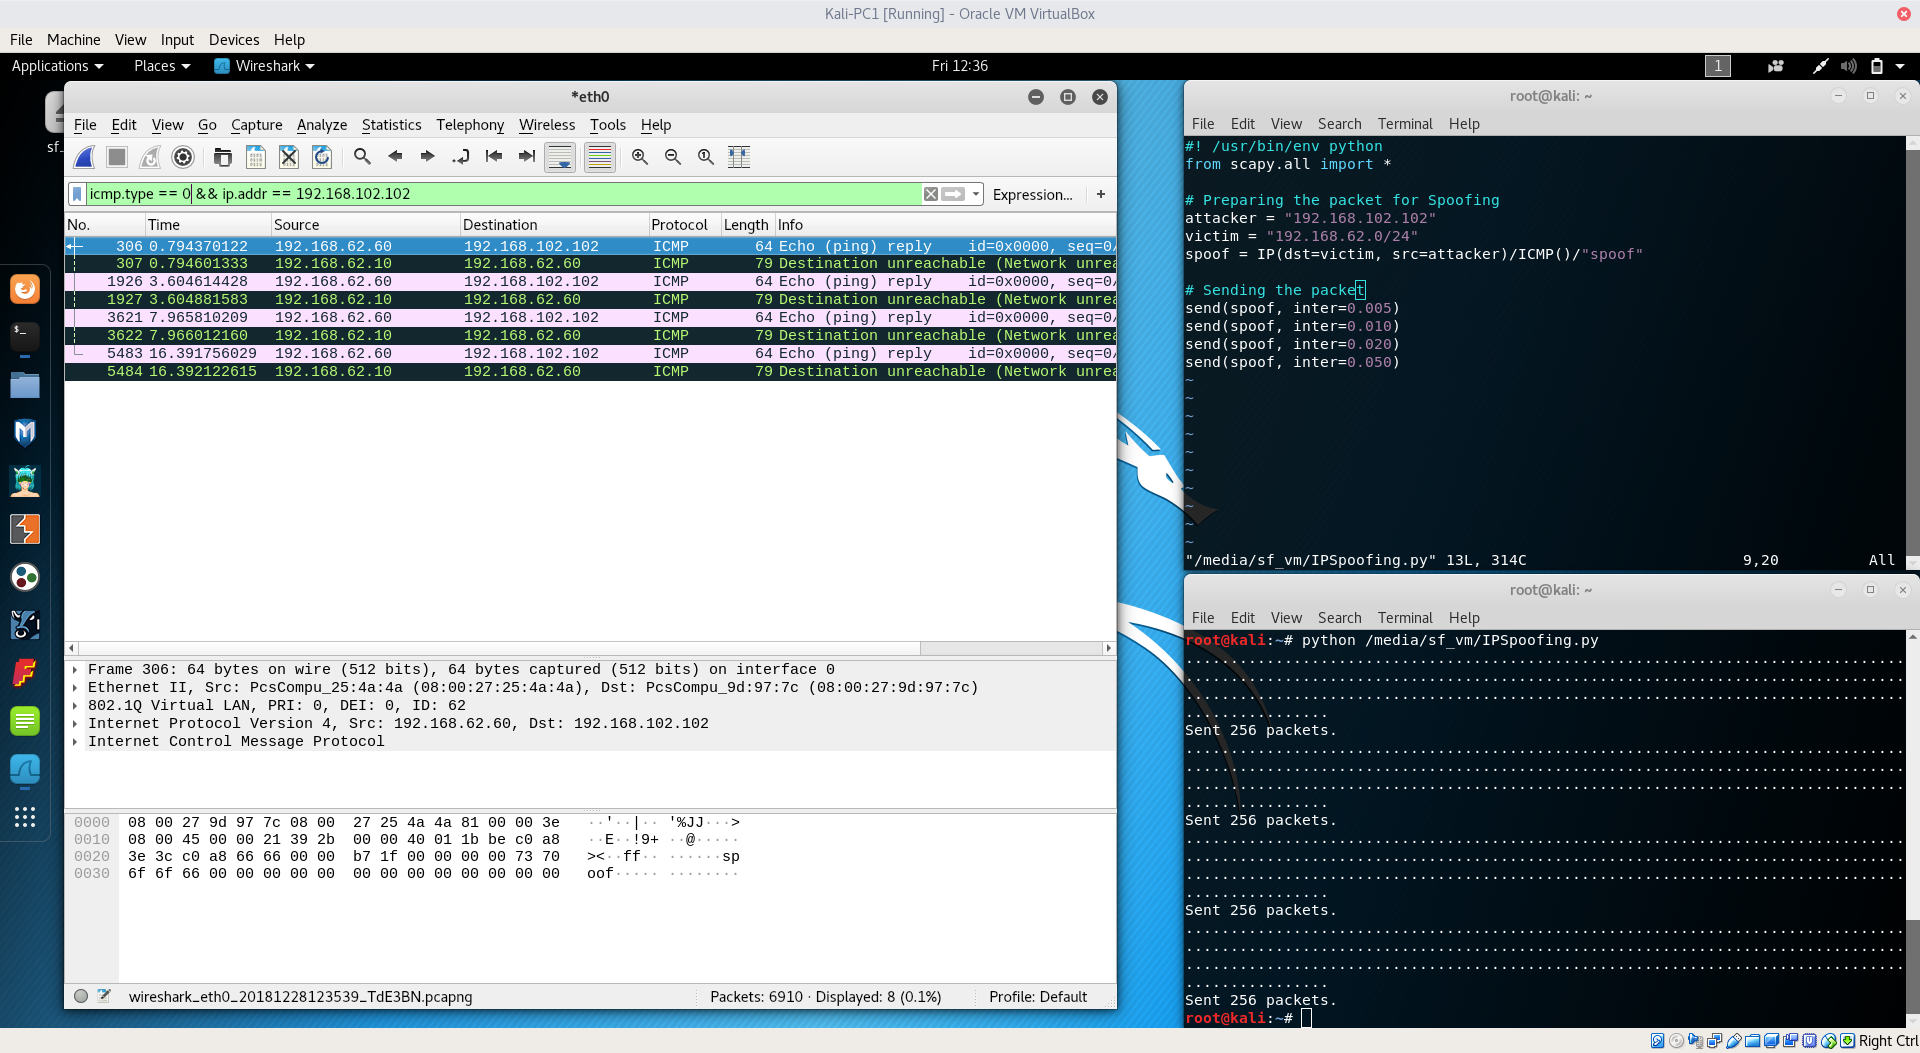
\includegraphics[width=16cm]{img/IPSpoofingReply.png}

% Method recommended to protect the Network against such an attack
\subsubsection{How to protect the network}
In order to protect the network a possible solution is to blocks all the incoming ICMP packets.
